\documentclass[tikz,border=4pt]{standalone}
\usepackage[T1]{fontenc}
\usepackage[utf8]{inputenc}
\usepackage{FiraSans}
\usepackage{amsmath}
\usetikzlibrary{arrows.meta,positioning,calc}
\definecolor{ceBlue}{RGB}{42,96,153}
\definecolor{ceTeal}{RGB}{36,135,118}
\definecolor{ceGold}{RGB}{220,160,52}
\definecolor{ceRed}{RGB}{188,74,60}
\definecolor{ceInk}{RGB}{42,42,42}
\definecolor{ceGray}{RGB}{238,240,242}
\begin{document}
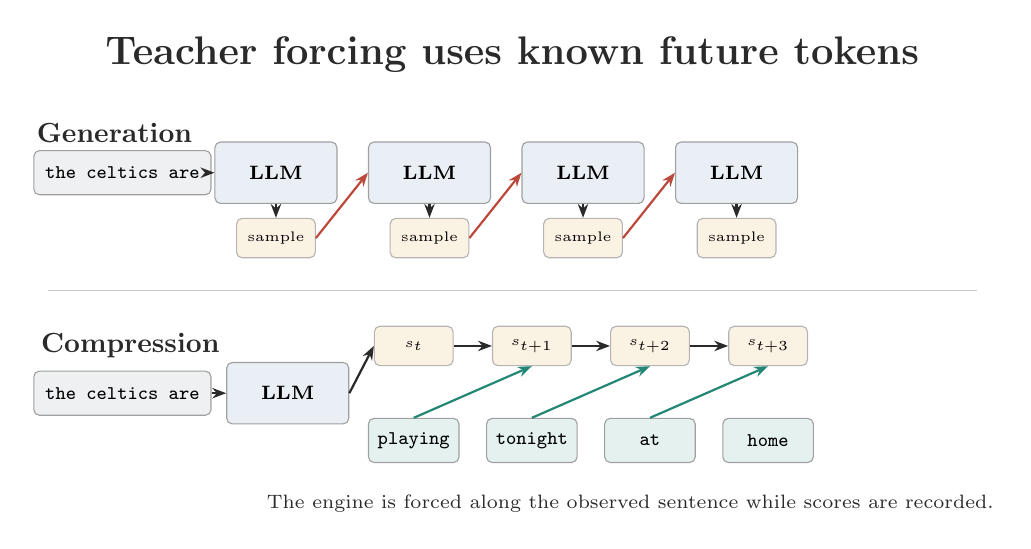
\begin{tikzpicture}[
  x=1cm,y=1cm,
  font=\sffamily,
  tok/.style={draw=ceInk!45, rounded corners=2pt, minimum width=1.15cm, minimum height=0.56cm, font=\scriptsize, fill=white},
  model/.style={draw=ceInk!45, rounded corners=2pt, minimum width=1.55cm, minimum height=0.78cm, font=\scriptsize\bfseries, fill=ceBlue!10},
  score/.style={draw=ceInk!35, rounded corners=2pt, minimum width=1.0cm, minimum height=0.5cm, font=\tiny, fill=ceGold!14},
  arr/.style={-{Stealth[length=5pt]}, thick, ceInk},
  feed/.style={-{Stealth[length=5pt]}, thick, ceTeal},
  sample/.style={-{Stealth[length=5pt]}, thick, ceRed},
]
  \node[font=\Large\bfseries, ceInk] at (6.5,6.05) {Teacher forcing uses known future tokens};

  \node[font=\bfseries, ceInk] at (1.45,5.05) {Generation};
  \node[tok, fill=ceGray, minimum width=2.25cm] (gctx) at (1.55,4.55) {\texttt{the celtics are}};
  \foreach \i/\x in {0/3.5,1/5.45,2/7.4,3/9.35} {
    \node[model] (g\i) at (\x,4.55) {LLM};
    \node[score] (gs\i) at (\x,3.72) {sample};
    \draw[arr] (g\i) -- (gs\i);
  }
  \draw[arr] (gctx) -- (g0);
  \foreach \i/\j in {0/1,1/2,2/3} {
    \draw[sample] (gs\i.east) -- (g\j.west);
  }

  \draw[ceInk!25] (0.6,3.05) -- (12.4,3.05);

  \node[font=\bfseries, ceInk] at (1.65,2.35) {Compression};
  \node[tok, fill=ceGray, minimum width=2.25cm] (p) at (1.55,1.75) {\texttt{the celtics are}};
  \node[model] (m) at (3.65,1.75) {LLM};
  \draw[arr] (p) -- (m);
  \foreach \i/\x/\lab in {0/5.25/$s_t$,1/6.75/$s_{t+1}$,2/8.25/$s_{t+2}$,3/9.75/$s_{t+3}$} {
    \node[score] (s\i) at (\x,2.35) {\lab};
  }
  \draw[arr] (m.east) -- (s0.west);
  \foreach \i/\j in {0/1,1/2,2/3} {
    \draw[arr] (s\i.east) -- (s\j.west);
  }
  \foreach \i/\x/\lab in {0/5.25/playing,1/6.75/tonight,2/8.25/at,3/9.75/home} {
    \node[tok, fill=ceTeal!12] (t\i) at (\x,1.15) {\texttt{\lab}};
  }
  \draw[feed] (t0.north) -- (s1.south);
  \draw[feed] (t1.north) -- (s2.south);
  \draw[feed] (t2.north) -- (s3.south);
  \node[font=\scriptsize, ceInk, align=center] at (8.0,0.35)
    {The engine is forced along the observed sentence while scores are recorded.};
\end{tikzpicture}
\end{document}
